%
% Methodology
%
\chapter{Methodology} \label{sec:methodology}
In this chapter we will propose several potential solutions to improve the performance of VGC-Bench's RL agents under non-stationarity.
We continue with the same problem statement and assumptions outlined in Chapter \ref{sec:preliminary}: We train an agent on regulation \textbf{A}, then on \textbf{B}, \textbf{C}, etc.
No regulation will be revisited after it is played, and no information about future regulations is available a priori.

Our first proposed improvement involves the policy architecture and the unstable behavior of the value function, as shown in Chapter \ref{sec:preliminary:analysis}.
While we initially used the same policy architecture as VGC-Bench (shown in Figure \ref{fig:vgcbench-architecture}), we now propose two minor adjustments to help stabilize the training of the value function:

\begin{enumerate}
    \item Change the Gaussian initialization of the item, move, and ability embeddings from $\mathcal{N}(0, 1)$ to $\mathcal{N}(0, 0.02)$. These embeddings receive sparse gradients, highly dependent on the items, moves, and abilities seen during training (with the majority never being seen at all). Additionally, these embeddings are suffering from vanishing gradients as they are placed at the very start of the network. Lowering the magnitude of the initialization makes the gradients more effective without drastically altering the original architecture. Despite this adjustment being in view of the value function, we apply this change to both the actor and the critic to keep their respective networks equivalent.
    \item Change the gain of the orthogonal initialization of the linear layer projecting the transformer output to the value prediction from 1 to 0.01. The large gain of the original initialization makes the initial value predictions biased and outside the $[-1, 1]$ range. Similarly to the embeddings, lowering the magnitude of the initialization reduces the effect of this bias and should make the learning of the value function more stable.
\end{enumerate}

With these two architectural adjustments to aid with the stability of the training process, we can now look into the various continual reinforcement learning methods outlined in Chapter \ref{sec:cl:crl}.

\textit{Regularization-based methods} identify parameters that are important for previously learned tasks and penalize changes to these parameters.
Alternatively, \textit{replay-based methods} store examples from previously encountered tasks and interleave them with new experiences during training.
While these methods could definitely have an impact in our problem setting, they are mainly focused on mitigating catastrophic forgetting and do not provide a clear solution to loss of plasticity~\cite{wang2024cl}.
Since in the scope of this thesis we explicitly state that no regulation will be revisited after it is played, we speculate that these methods will have less of an impact than methods that explicitly mitigate loss of plasticity.

\textit{Parameter-isolation methods} allocate separate subsets of model parameters to different tasks, providing a clear solution to loss of plasticity.
Progressive architectures like PNNs and PathNet are prime candidates for combining the plasticity of complete retraining with the knowledge retention of fine-tuning, though they will first have to be adapted to transformer models for VGC-Bench's policy architecture.
While LoRA is a compelling method that serves this purpose, it is more intended for large transformer models that cannot easily be fine-tuned, something that we already showed is possible for VGC-Bench's policy architecture in Chapter \ref{sec:preliminary:finetune}~\cite{hu2022lora}.

Other options for mitigating loss of plasticity include  specialized optimization methods like ReDo and Continual Backprop.
While these methods were explicitly created to combat loss of plasticity, recent work by \textcite{dohare2024plasticity} showed that they have a limited benefit over a tuned version of PPO in the context of continual reinforcement learning.
Combined with the fact that these methods have not yet been adapted for transformer models, we speculate that \textcite{dohare2024plasticity}'s tuned PPO will be able to give us more consistent results.

\section{Progressive Architecture} \label{sec:progressive}
Progressive neural networks are an established continual learning method that allocates separate 'columns' of a network to different tasks.
Each column has lateral connections to previous columns, allowing the network to reuse previously learned representations~\cite{rusu2016pnn}.
By introducing new weights for every task, PNNs effectively remove the issue of loss of plasticity.
For this reason, we believe that a progressive architecture could help improve the performance of VGC-Bench's RL agents under non-stationarity.

When adapting VGC-Bench's policy architecture to a progressive variant, we base our work on \textcite{rusu2016pnn}'s original PNN architecture, allocating separate columns for every regulation.
If network size becomes an issue we could consider switching to PathNet, an alternative to PNNs that operates on a fixed-size network~\cite{fernando2017pathnet}, but with only 10 regulations we do not foresee this becoming an issue.

\begin{figure}[ht]
    \centering
    \begin{subfigure}{.95\textwidth}
        \centering
        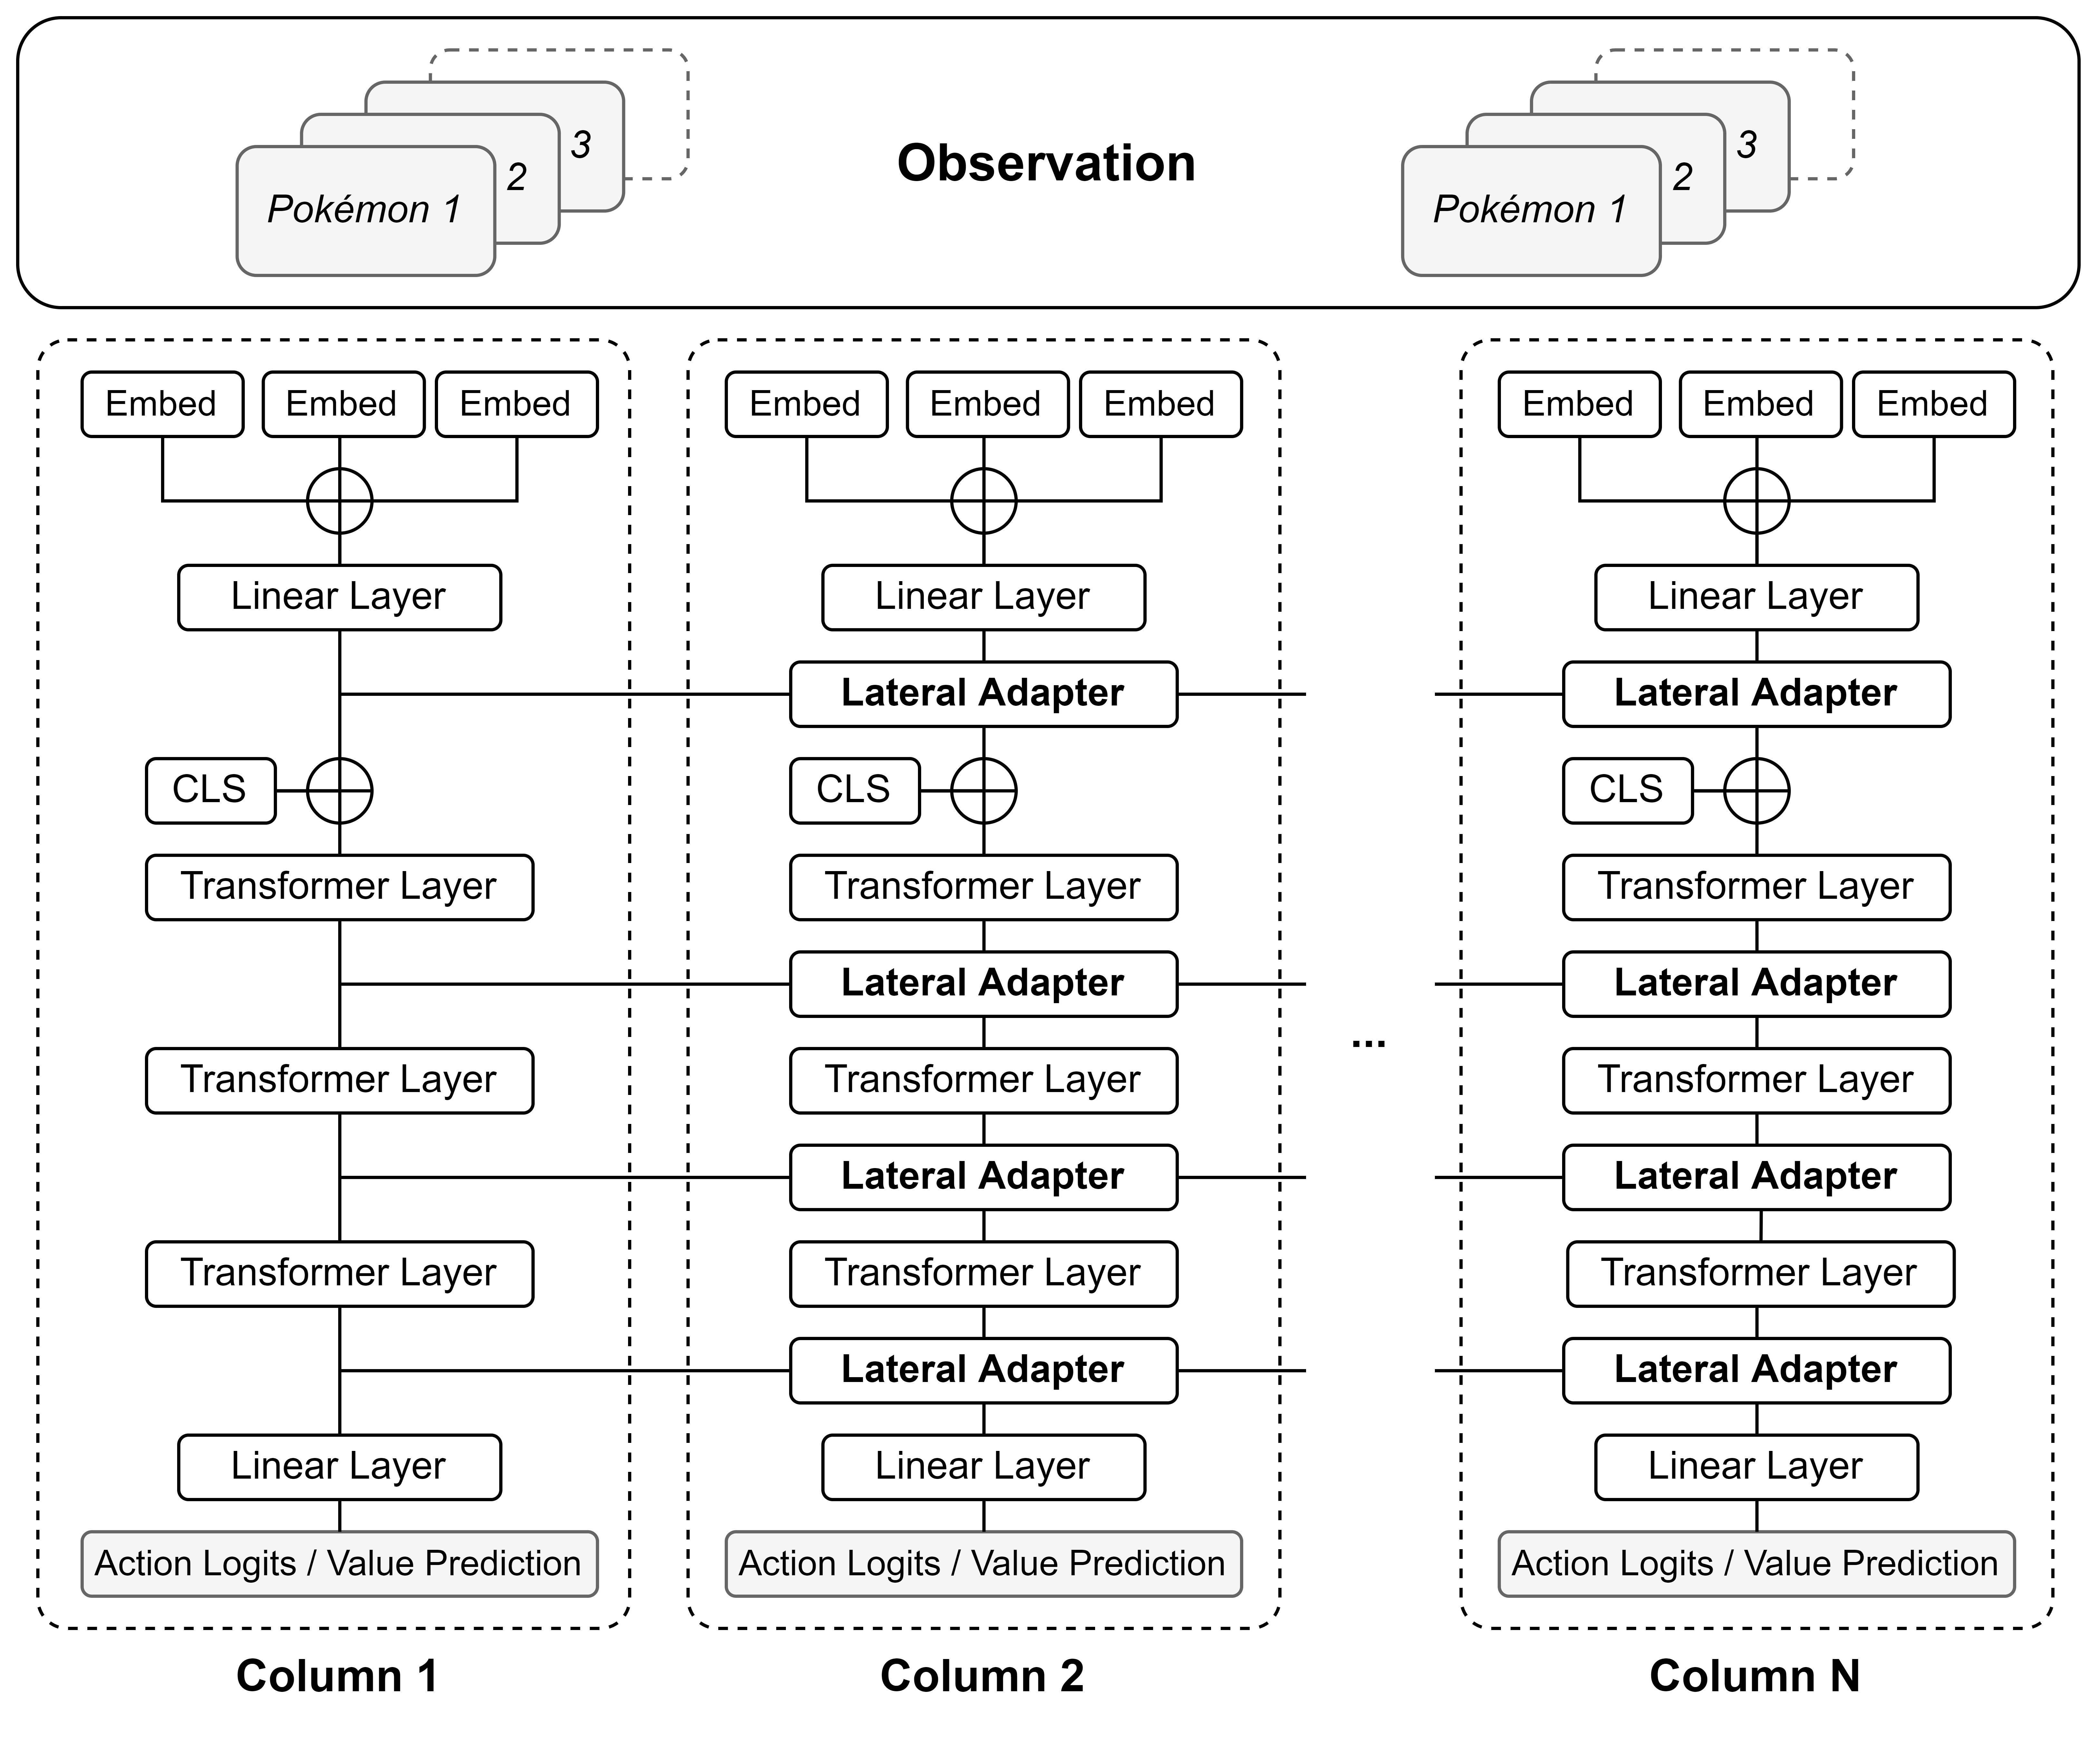
\includegraphics[width=\textwidth]{images/figures/progressive.png}
        \caption{Our proposed progressive architecture.}
        \label{fig:progressive:architecture}
    \end{subfigure}
    \par\bigskip
    \begin{subfigure}{.65\textwidth}
        \centering
        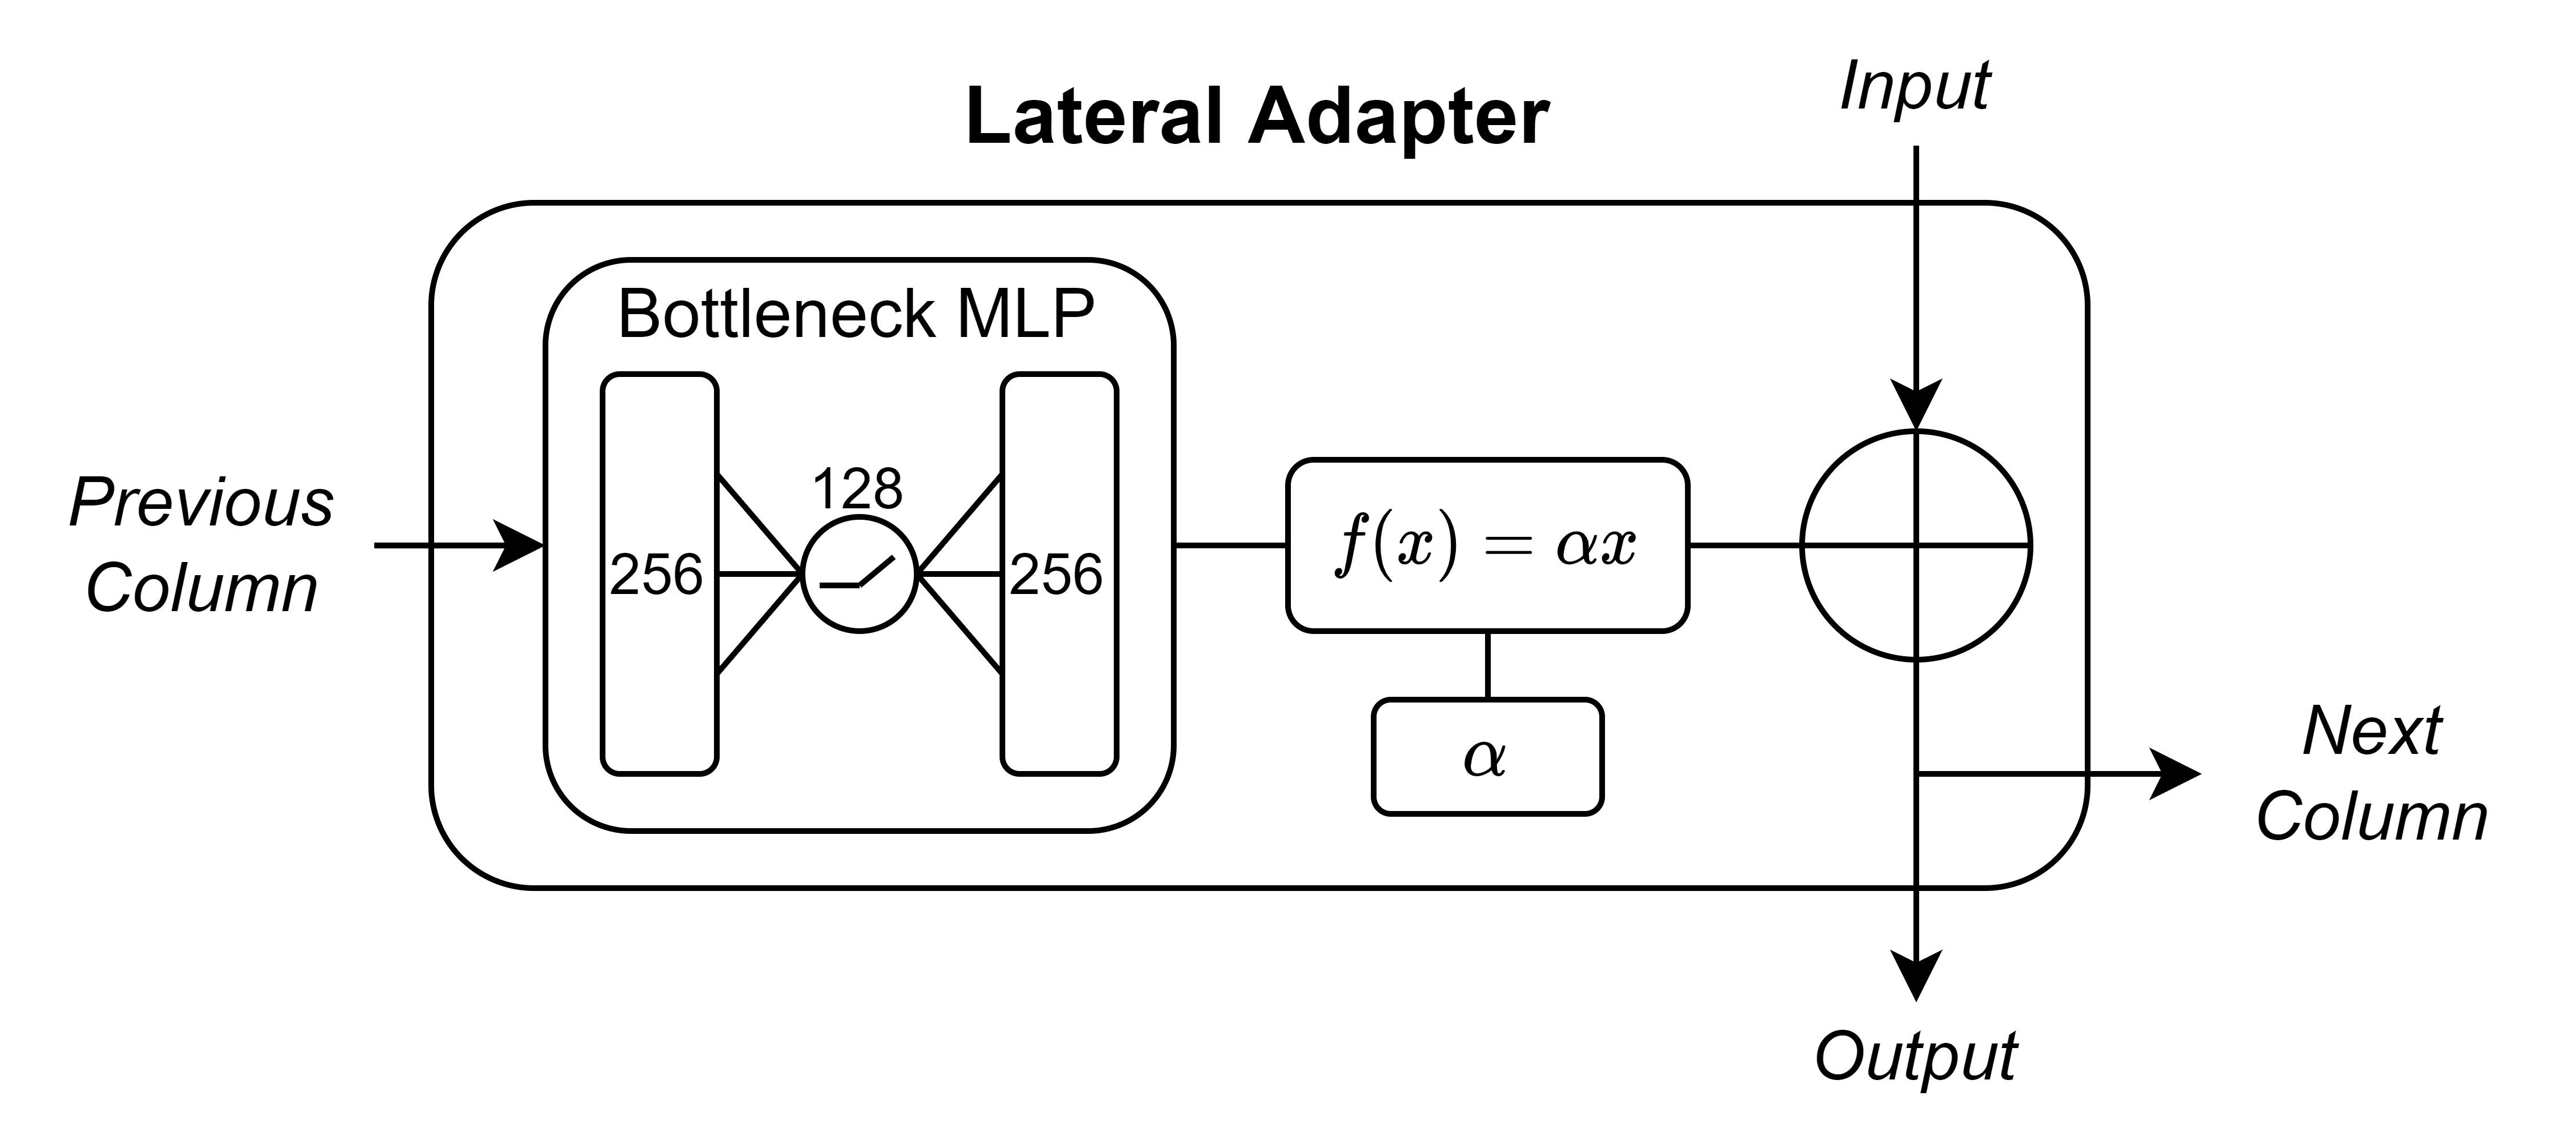
\includegraphics[width=\textwidth]{images/figures/lateral-adapter.png}
        \caption{The lateral adapter connecting adjacent columns.}
        \label{fig:progressive:adapter}
    \end{subfigure}
    \caption{VGC-Bench's policy architecture (see Figure \ref{fig:vgcbench-architecture}), adapted to a progressive variant with columns for regulations. Both actor and critic use the same architecture with separate columns and no direct parameter sharing.}
    \label{fig:progressive}
\end{figure}

Figure \ref{fig:progressive} shows our proposed adaptation of VGC-Bench's policy architecture to a progressive variant with columns for each regulation.
When a new column is added, the previous column's weights are frozen and stop receiving gradients.
We only use the action logits and value predictions of the column corresponding to the current regulation.
We identify four potential lateral transfer points: One after the feature aggregation, and one after each of the three transformer layers.
These transfer points feel closest in line to the original PNN architecture by \textcite{rusu2016pnn}, which transfers laterally after every network layer~\cite{rusu2016pnn}.

At each transfer point, the lateral signal from the previous column is combined with the current column's signal through a lateral adapter (shown in Figure \ref{fig:progressive:adapter}).
The lateral signal first passes through two linear layers arranged as a bottleneck, restricting the signal to half of its original dimensions and forcing it to a more robust representation.
It is then scaled by a learned vector $\alpha = (\alpha_1, \alpha_2, ... , \alpha_{256})$ before being added to the current column's signal.
This output signal is then passed to the rest of the current column or as lateral signal to the next column.

One adjustment we make compared to the original PNN architecture is that each column only provides a lateral signal to its next adjacent column, instead of all future columns~\cite{rusu2016pnn}.
This changes the growth of the network from exponential to linear, making it more compact while representations from column $i$ can still transfer to column $i + n$ through the cascading structure of lateral adapters.

\FloatBarrier

\section{Tuned PPO} \label{sec:tuned}
Rather than adapting specialized optimization methods like ReDo or Continual Backprop to transformer models, we are instead more interested in the tuned version of PPO, introduced by \textcite{dohare2024plasticity}, that achieves very similar results in continual reinforcement learning settings.

The main adjustment this tuned version makes is to the $\beta_1$ and $\beta_2$ parameters of the Adam optimizer, which relate to the optimizer's running estimate of the gradient and the squared gradient respectively.
The standard values of $\beta_1$ and $\beta_2$ used by the Adam optimizer (and PPO by extension) are 0.9 and 0.999 respectively.
\textcite{lyle2023plasticity} showed that these standard values cause a large loss of plasticity, caused by the fact that $\beta_1 \neq \beta_2$.
A large value of $\beta_2$ means that the running estimate for the squared gradient, used in the denominator, is updated much more slowly than the running estimate for the gradient, used in the numerator~\cite{dohare2024plasticity,lyle2023plasticity}.
\textcite{lyle2023plasticity} proposed setting $\beta_1 = \beta_2 = 0.99$, resulting in smaller updates that lead to a more stable training.

\textcite{dohare2024plasticity} used this tuned version of the Adam optimizer combined with PPO and L2 regularization as a baseline for ReDo and Continual Backprop in a continual reinforcement learning setting, referring to it as \textit{``tuned PPO"}.
While tuned PPO performed worse than Continual Backprop in stationary environments, it was able to keep up in non-stationarity environments, only falling 1-2\% percent behind in terms of reward while vastly outperforming regular PPO~\cite{dohare2024plasticity}.
For this reason, we believe that tuned PPO could help improve the performance of VGC-Bench's RL agents under non-stationarity.

We replicate \textcite{dohare2024plasticity}'s tuned PPO by updating the Adam optimizer's $\beta$'s to $\beta_1 = \beta_2 = 0.99$ and by enabling L2 regularization, both for training and for fine-tuning.
The only adjustment we make has to do with the L2 regularization rate $\lambda$: Whereas \textcite{dohare2024plasticity} use a rate of 1e-5, we opt for a more conservative 1e-6.
